Through the course of these experiments, we have learned a number of lessons pertaining to the behavior of Spark at large scale. In this section, we share some of these lessons and conjecture on likely causes.
\subsection{Spark Sequential Bottlenecks}

\begin{table}[th]
\begin{center}
\resizebox{\columnwidth}{!}{
\begin{tabular}{| c | c | c | c | c | c | c |}
\hline
Algo & Size & Nodes & Partitions & Time (s) & Measured & Predicted \\
{} & {} & {} & {} & {} & Task Start & Delay \\
{} & {} & {} & {} & {} & Delay (s) & (2000/sec) \\
\hline
%\multirow{3}{*}{NMF} & \multirow{3}{*}{1.6 TB} & 
% 50 & 3200 & 710 & & \\
% {} & {} & 100 & 3200 & 457 & & \\
% {} & {} & 300 & 9600 & 215 & & \\ %\hline
\multirow{4}{*}{PCA} & \multirow{3}{*}{2.2 TB} & 100 & 3200 & 958 & 411 & 112 \\
 {} & {} & 300 & 9600 & 870 & 332 & 336 \\
 {} & {} & 500 & 16000 & 1232 & 542 & 560 \\ \cline{2-7} & & & & & & \\[-1ex]
 {} & {16 TB} & 1522 & 51200 & 3718 & 1779 & 1792 \\
 \hline
\end{tabular}
}
\end{center}
\caption{Spark scheduling delays}
\label{tab:scheduling}
\end{table}
There are two main sources of sequential bottleneck in Spark: Task Start Delay and Scheduler Delay. Task Start delay for a particular task is the time from the start of the stage to when the scheduler creates and sends out the task to an executor. Because tasks are created one by one by the driver as it checks resources to see where to send them, higher concurrency leads to high task start delays. Scheduler delay consists of two items: the time it takes for the executor to receive the message to start as task and spawn a thread and the time it takes for the task to send a message back to the driver. Scheduler delay is known to be either caused by large tasks or large results, which slow down the sending process. In our case, however, we believe that a big part of the scheduler delay we observe increasing as we increase concurrency is due to the large number of tasks we are launching at once. This causes delay as many task completed messages are sent back to the driver at once and are queued as they are processed one by one. Ousterhout et al~\cite{Ousterhout13Sparrow} showed that the Spark scheduler is limited to launching approximately 1500 tasks per second.  Their measurements were based on an older version of Spark from 2013.  There have not been significant changes to the scheduler, however, and our results on Cori are consistent with a similar rate of approximately 2000 tasks per second.  
In figure~\ref{fig:hero-timeline}, we show timeline of when tasks from the PCA hero run for a certain stage on a certain node are scheduled and what they spend time on. We can see that this sequential bottleneck causes a uniform distribution start times, with tasks starting as late as 20 seconds after the earliest task. Interestingly enough, the tasks finish at about the same time, as the scheduler delay seems to inversely proportional to the start delay. \textcolor{blue}{Adi, Alex:}
\begin{itemize}
\item \textcolor{blue}{Should we mention this weird behavior and just say we are not sure why }
\end{itemize}
Despite this strange behavior, it is clear that this delay negatively affects task performance. We show this impact in Table~\ref{tab:scheduling}.  

We expect the largest impact here, due to PCA being an iterative algorithm and the need to schedule 70 separate iterations, each of which contain a stage with the as many tasks as the partitions shown . The \emph{Partitions} column shows the number of data partitions (and thus tasks per full stage).\footnote{In order to minimize the impact of this bottleneck, we set the number of partitions to the exact number of cores allocated to each run.}  The \emph{Measured Task Start Delay} column shows the sum of the largest task start delays in each Spark stage.  The \emph{Predicted Delay} column shows the delay predicted by a scheduling rate of 2000 tasks per second.  This is obtained by multiplying the number of partitions by the 70 large initial tree aggregation stages (the smaller second stage of the tree aggregation has too few partitions for this delay to have a noticeable impact).  We observe that at 300 and 500 nodes (for the 2.2 TB dataset), and 1522 nodes (for the 16 TB dataset), the task start delay is very close to the value predicted. 

At 100 nodes, we see a delay that is much higher than predicted, indicating that an additional source of delay may have contributed.  In particular, there was a single task with a delay of 90 seconds during that run, which alone accounts for almost a third of the difference from the predicted value.

This bottleneck represents a limit on the scaling achievable by Spark for highly iterative algorithms.  In particular, as the amount of parallelism increases, the minimum number of partitions and tasks also increases.  This results in a linearly increasing overhead from the scheduler as we increase parallelism.  This delay is further multiplied by the number of stages (or, in the case of actions like a tree aggregation, the number of stages which operate on every partition).  We see the impact of this in the PCA results in Table~\ref{tab:scheduling}, where the final column represents this fixed overhead and is thus a limit on how fast we could possibly execute at the given scale.  
\subsection{Other Significant Spark Overheads}

\subsection{Spark variability}
During initial testing runs of the Spark PCA algorithm, variations in run time as large as 25\% were observed (in our staging runs we had a median run time of 645 seconds, a minium run time of 489 seconds, and a maximum run time of 716 seconds). These variations could not be attributed to any particular spark stage. Sometimes the delay would occur in the Multiply Gramian step, other times in the intial data collect stage. This variability is illustrated in the box and whiskers plot. Spark has a ``speculation" functionality which is aimed at reducing this variability somewhat. However, we found that turning the functionality on had no appreciable effect on improving the run time because the overhead to fetch an RDD from another worker was sufficiently high. This is because requests for RDDs from other workers must wait until the worker finishes its running tasks. This can often result in delays that are as long as the run time of the straggling task.  


\textcolor{blue}{Evan:}
\begin{itemize}
\item \textcolor{blue}{Do we know anything more about the 90 second delayed task in PCA 100 nodes from your email this morning?  If so we should mention it in the second paragraph of this section.}
\end{itemize}



\begin{figure}[t]
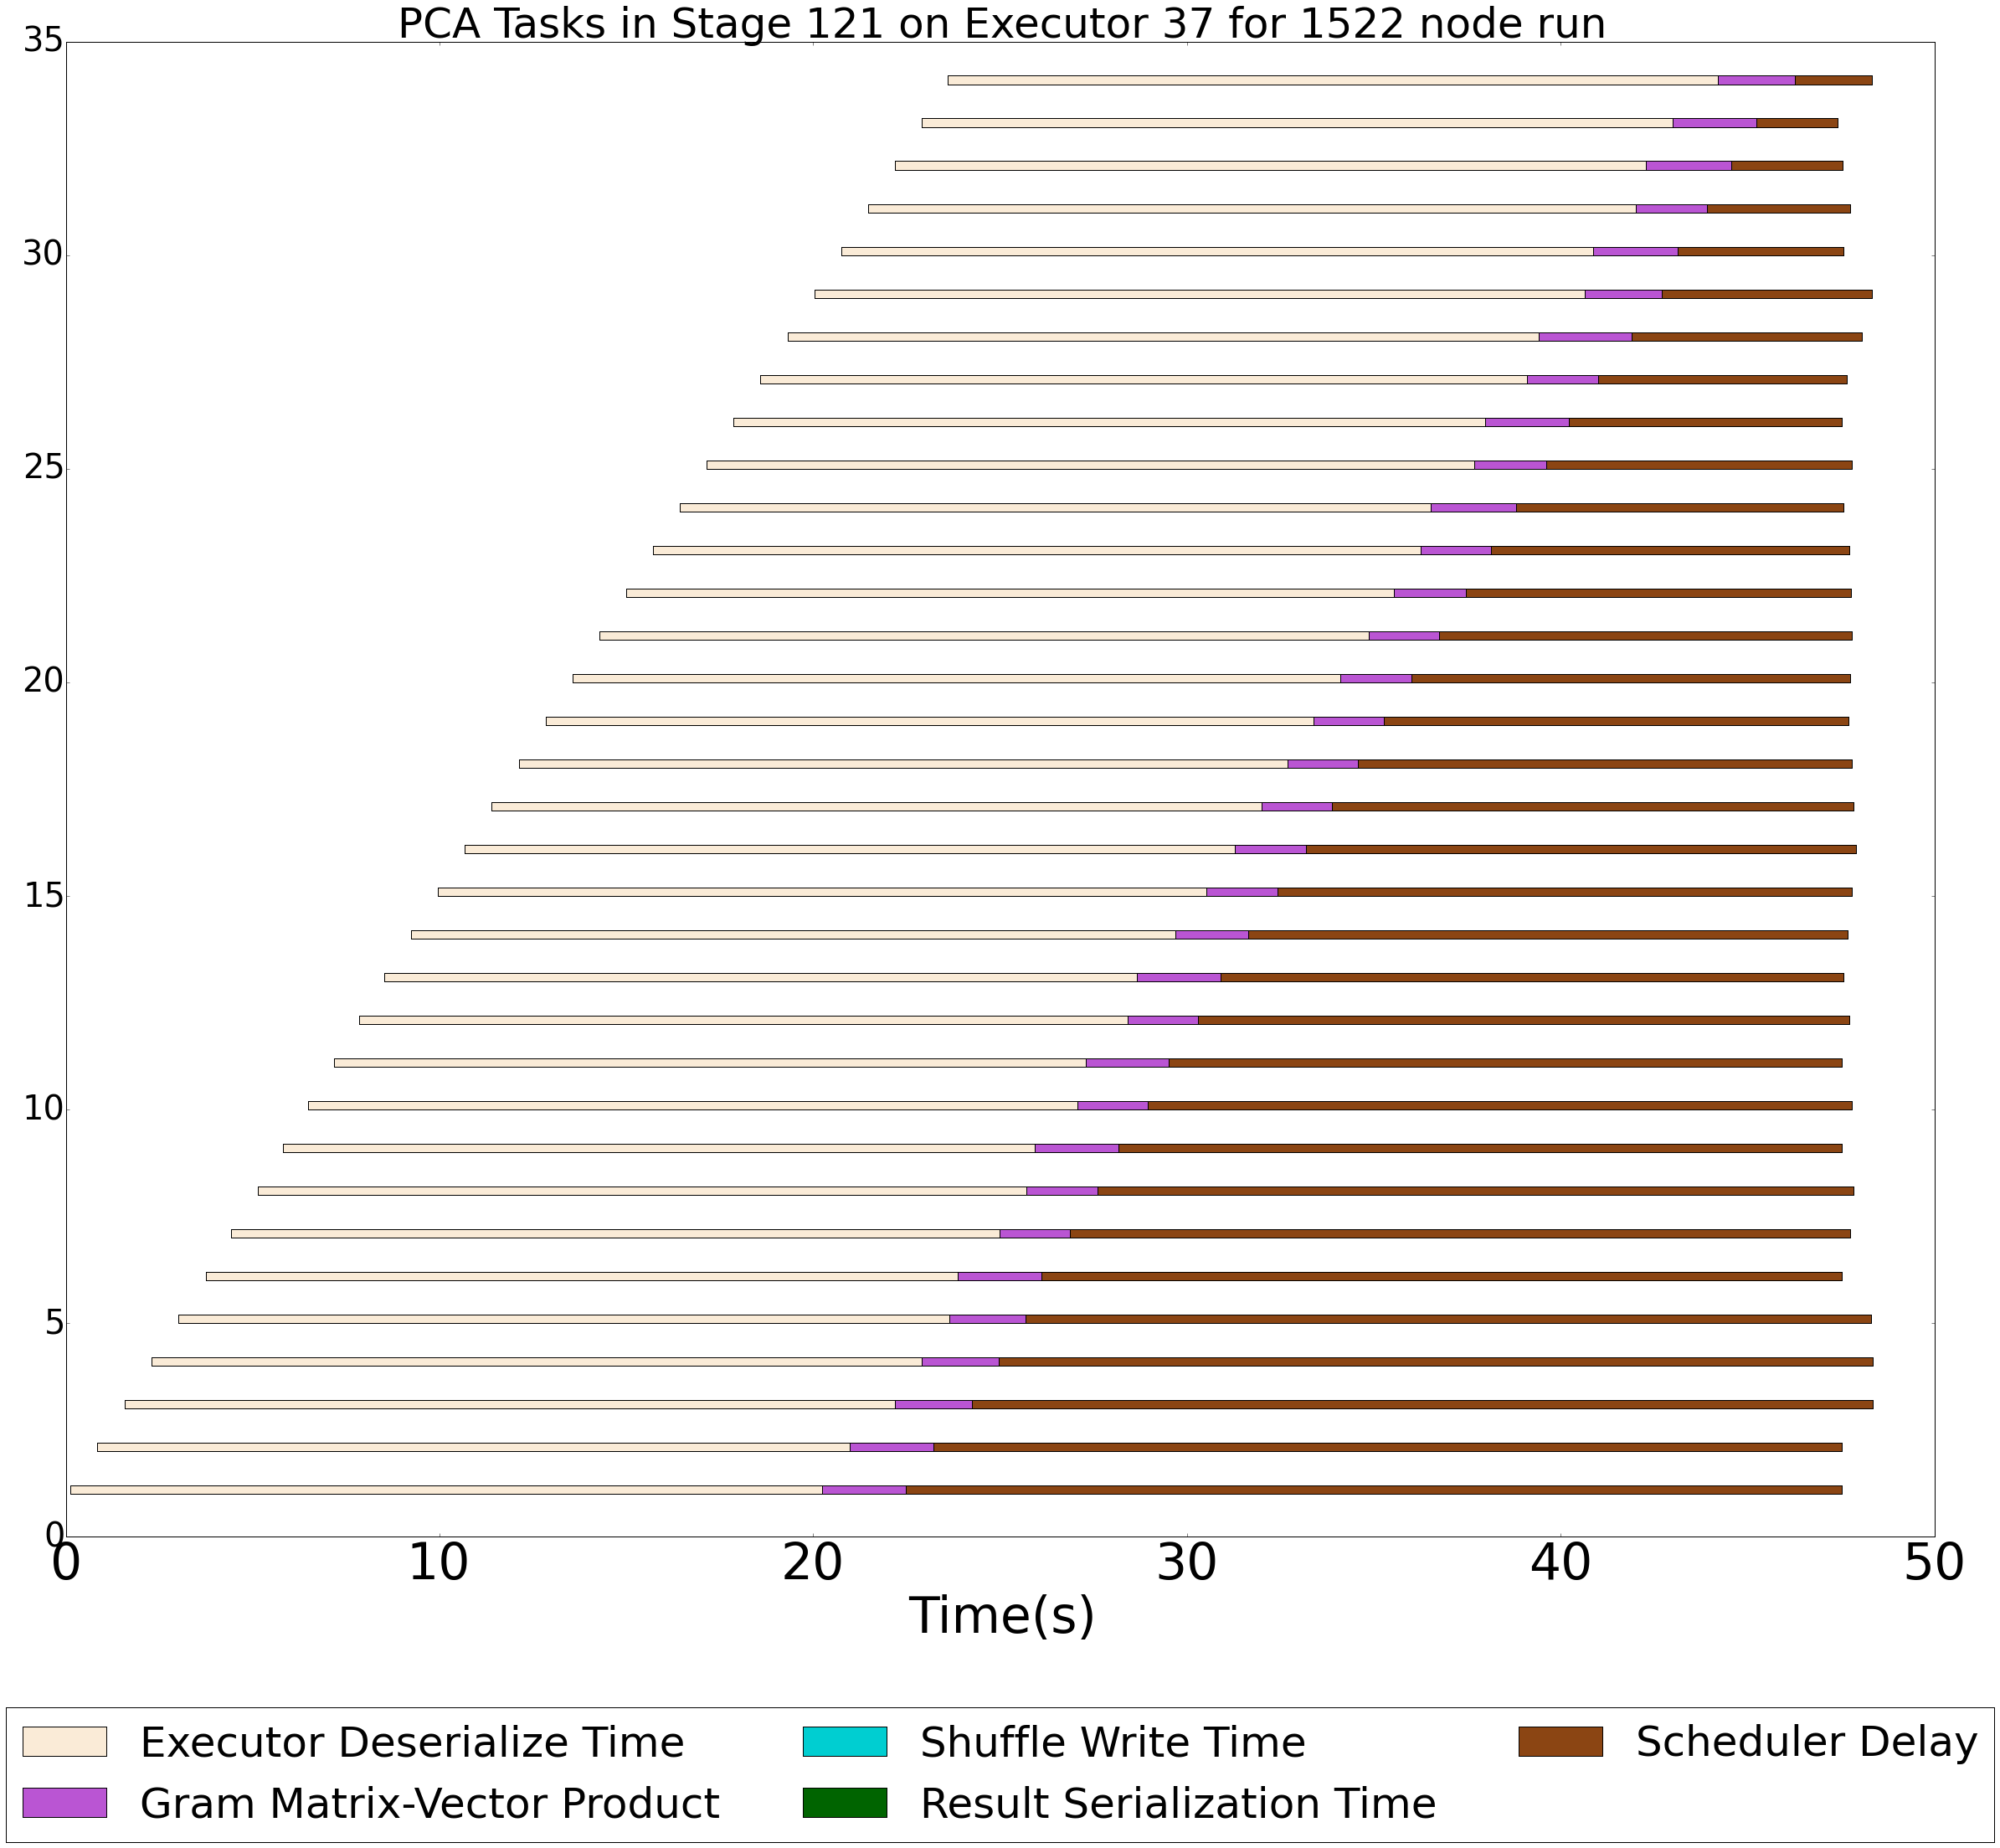
\includegraphics[width=.5\textwidth]{fig/spark_pca_hero_timeline.png}
\caption{A timeline a tasks on one node for a multiply gramian stage during the 1522 node Spark run }
\label{fig:hero-timeline}
\end{figure}

% \begin{figure}[t]
% 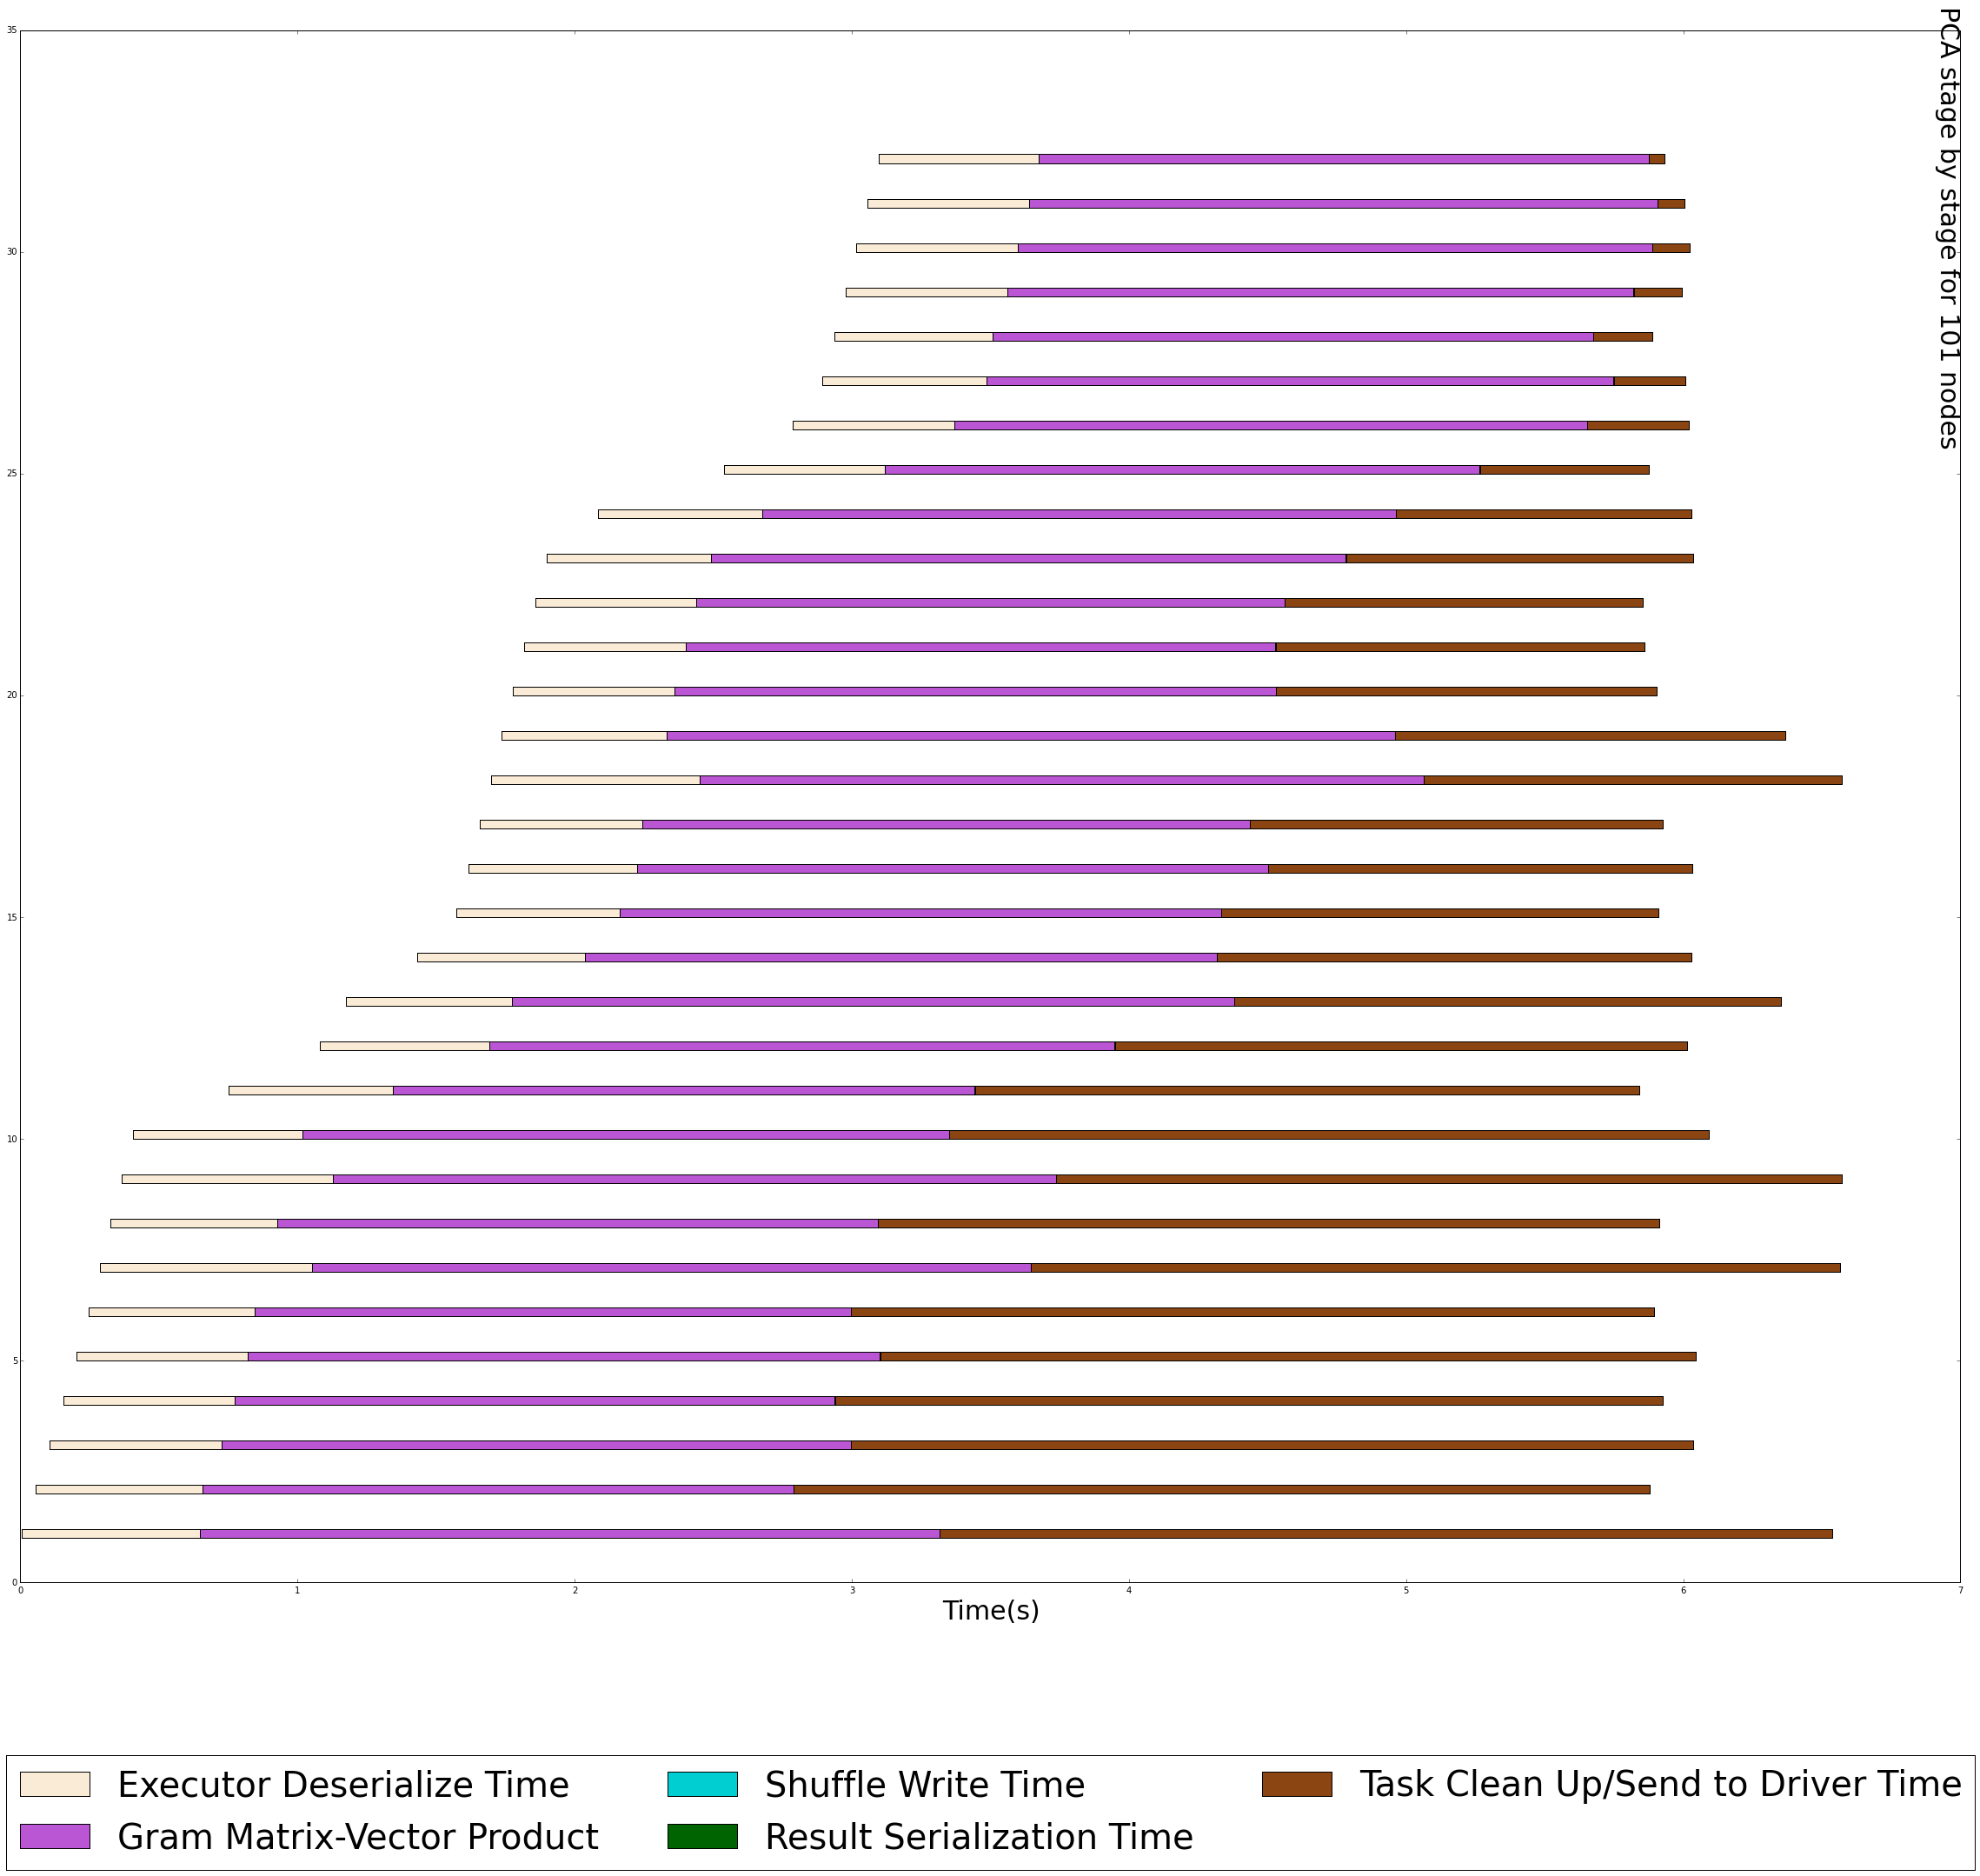
\includegraphics[width=.5\textwidth]{fig/pca_100_timeline.png}
% \caption{???}
% \label{fig:tofix-1}
% \end{figure}

% \begin{figure}[t]
% 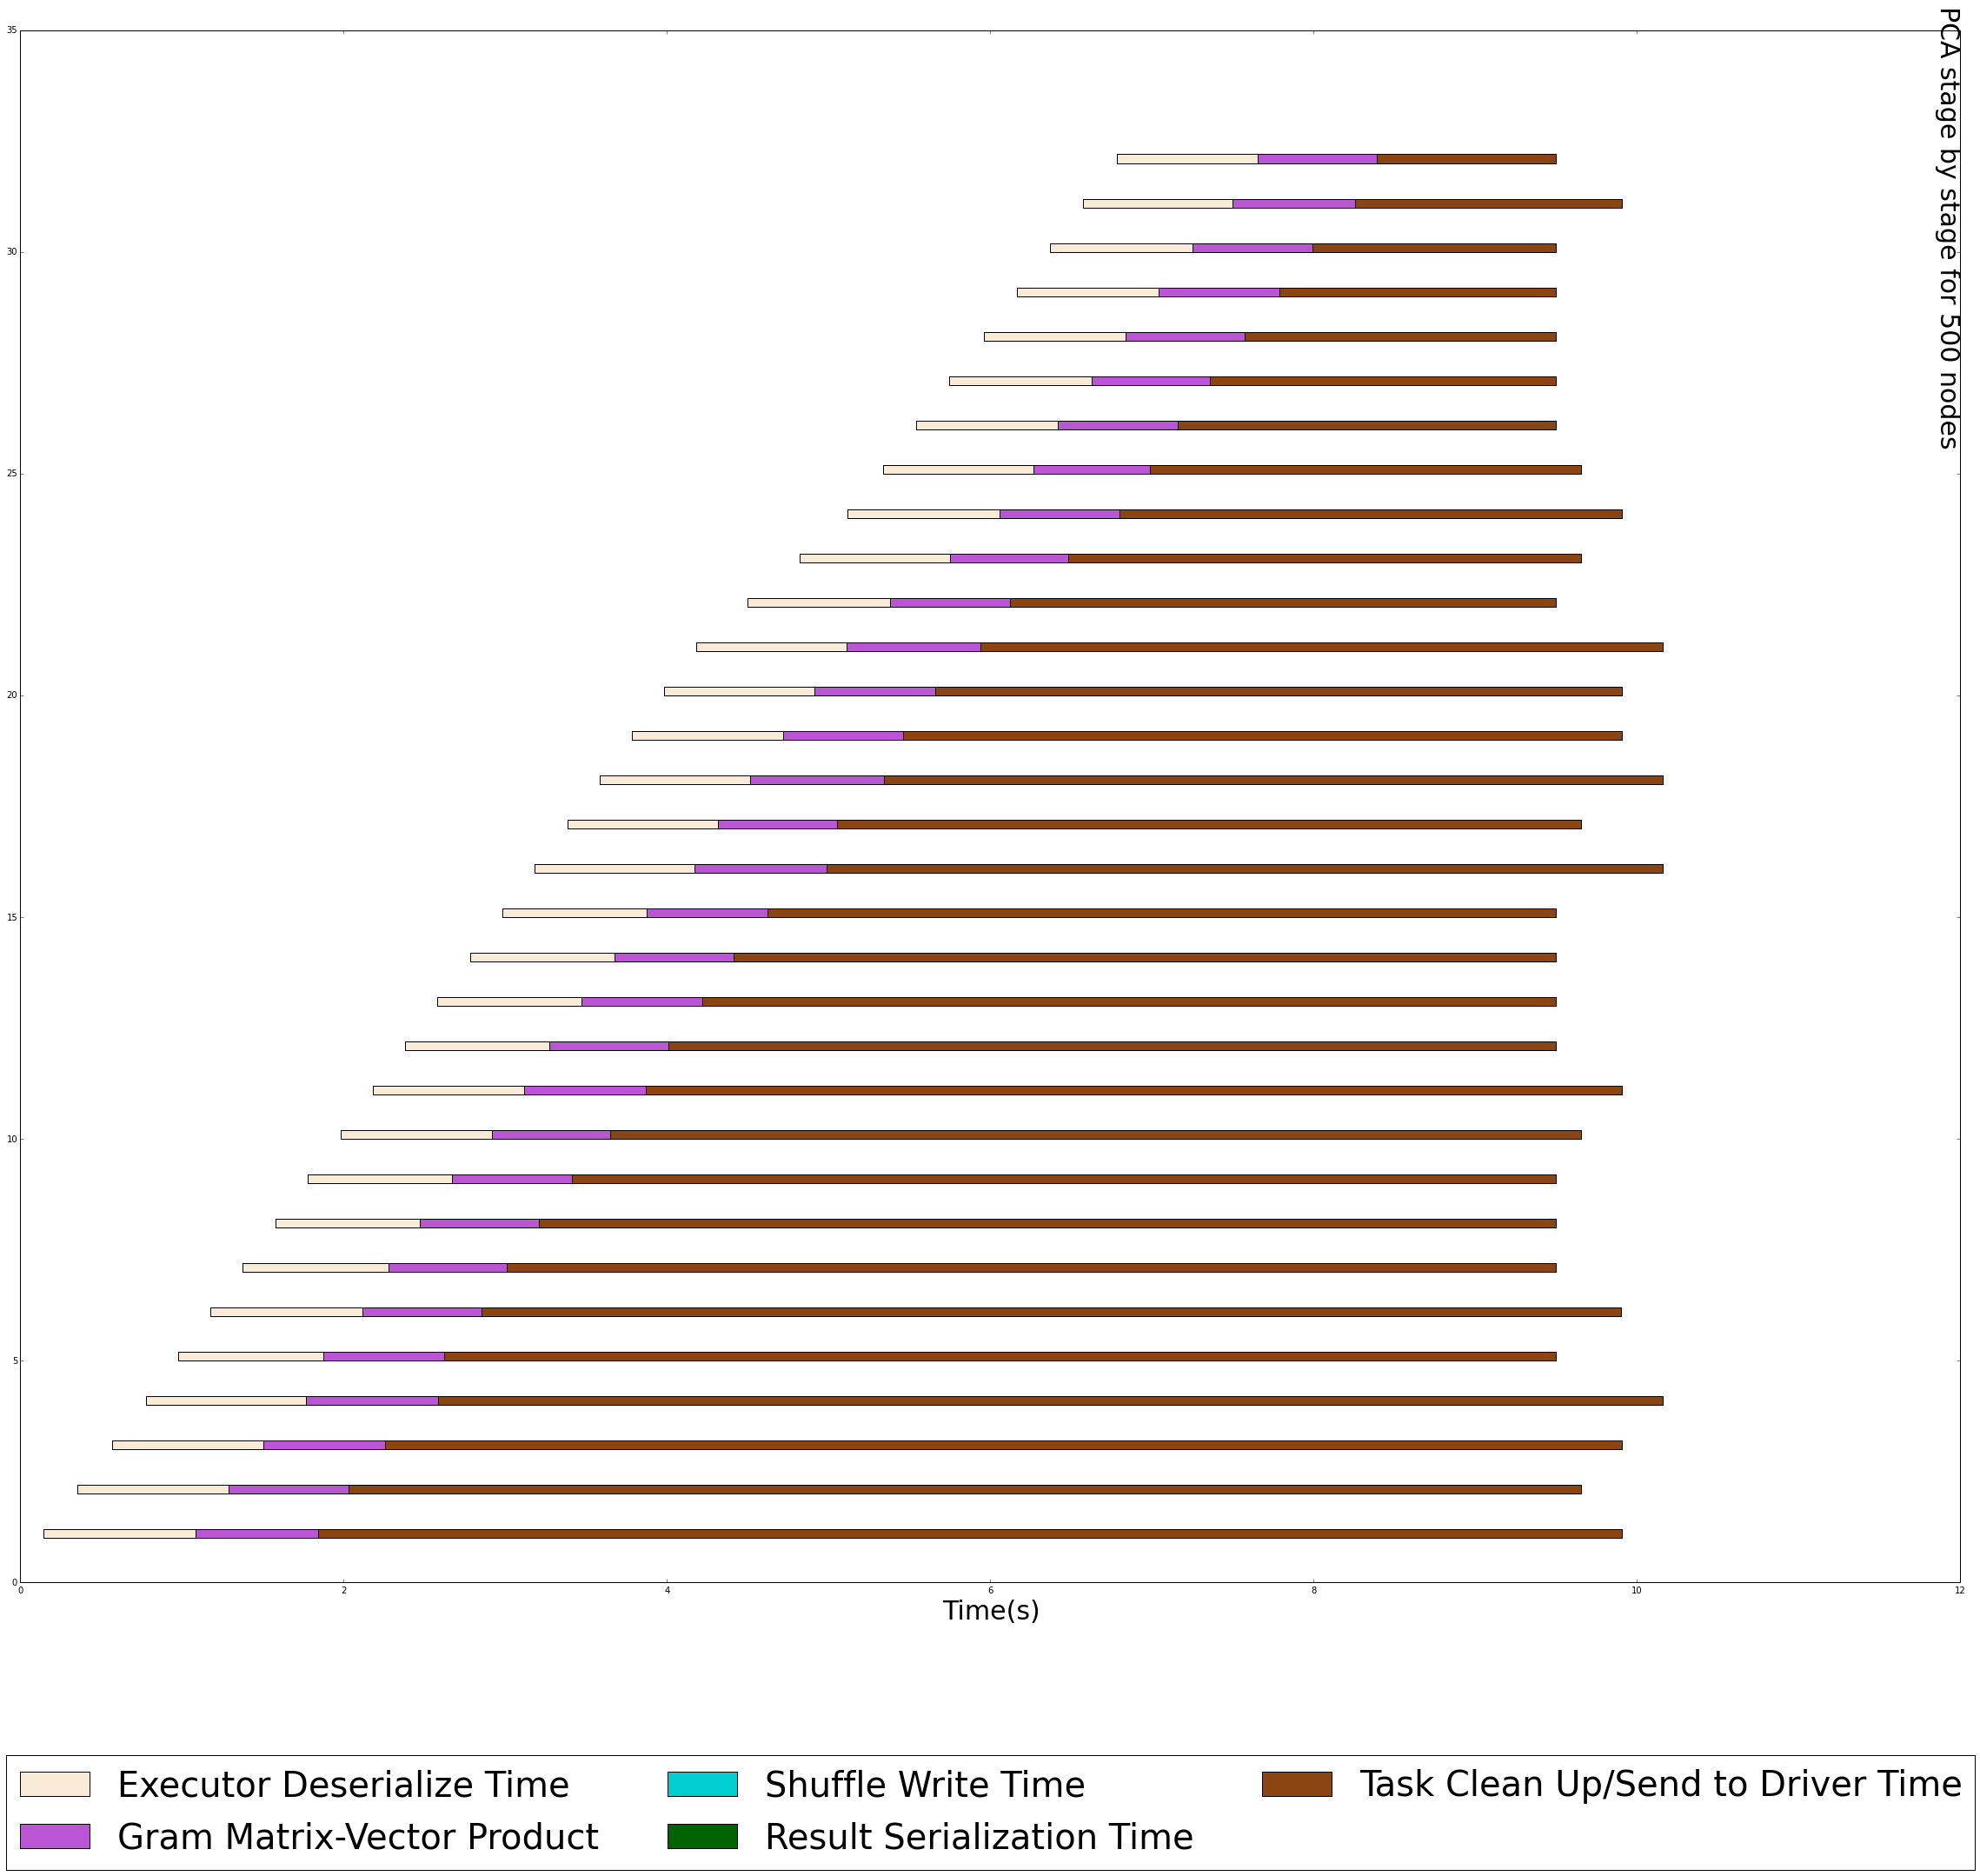
\includegraphics[width=.5\textwidth]{fig/pca_500_timeline.png}
% \caption{???}
% \label{fig:tofix-2}
% \end{figure}

% \begin{figure}[t]
% 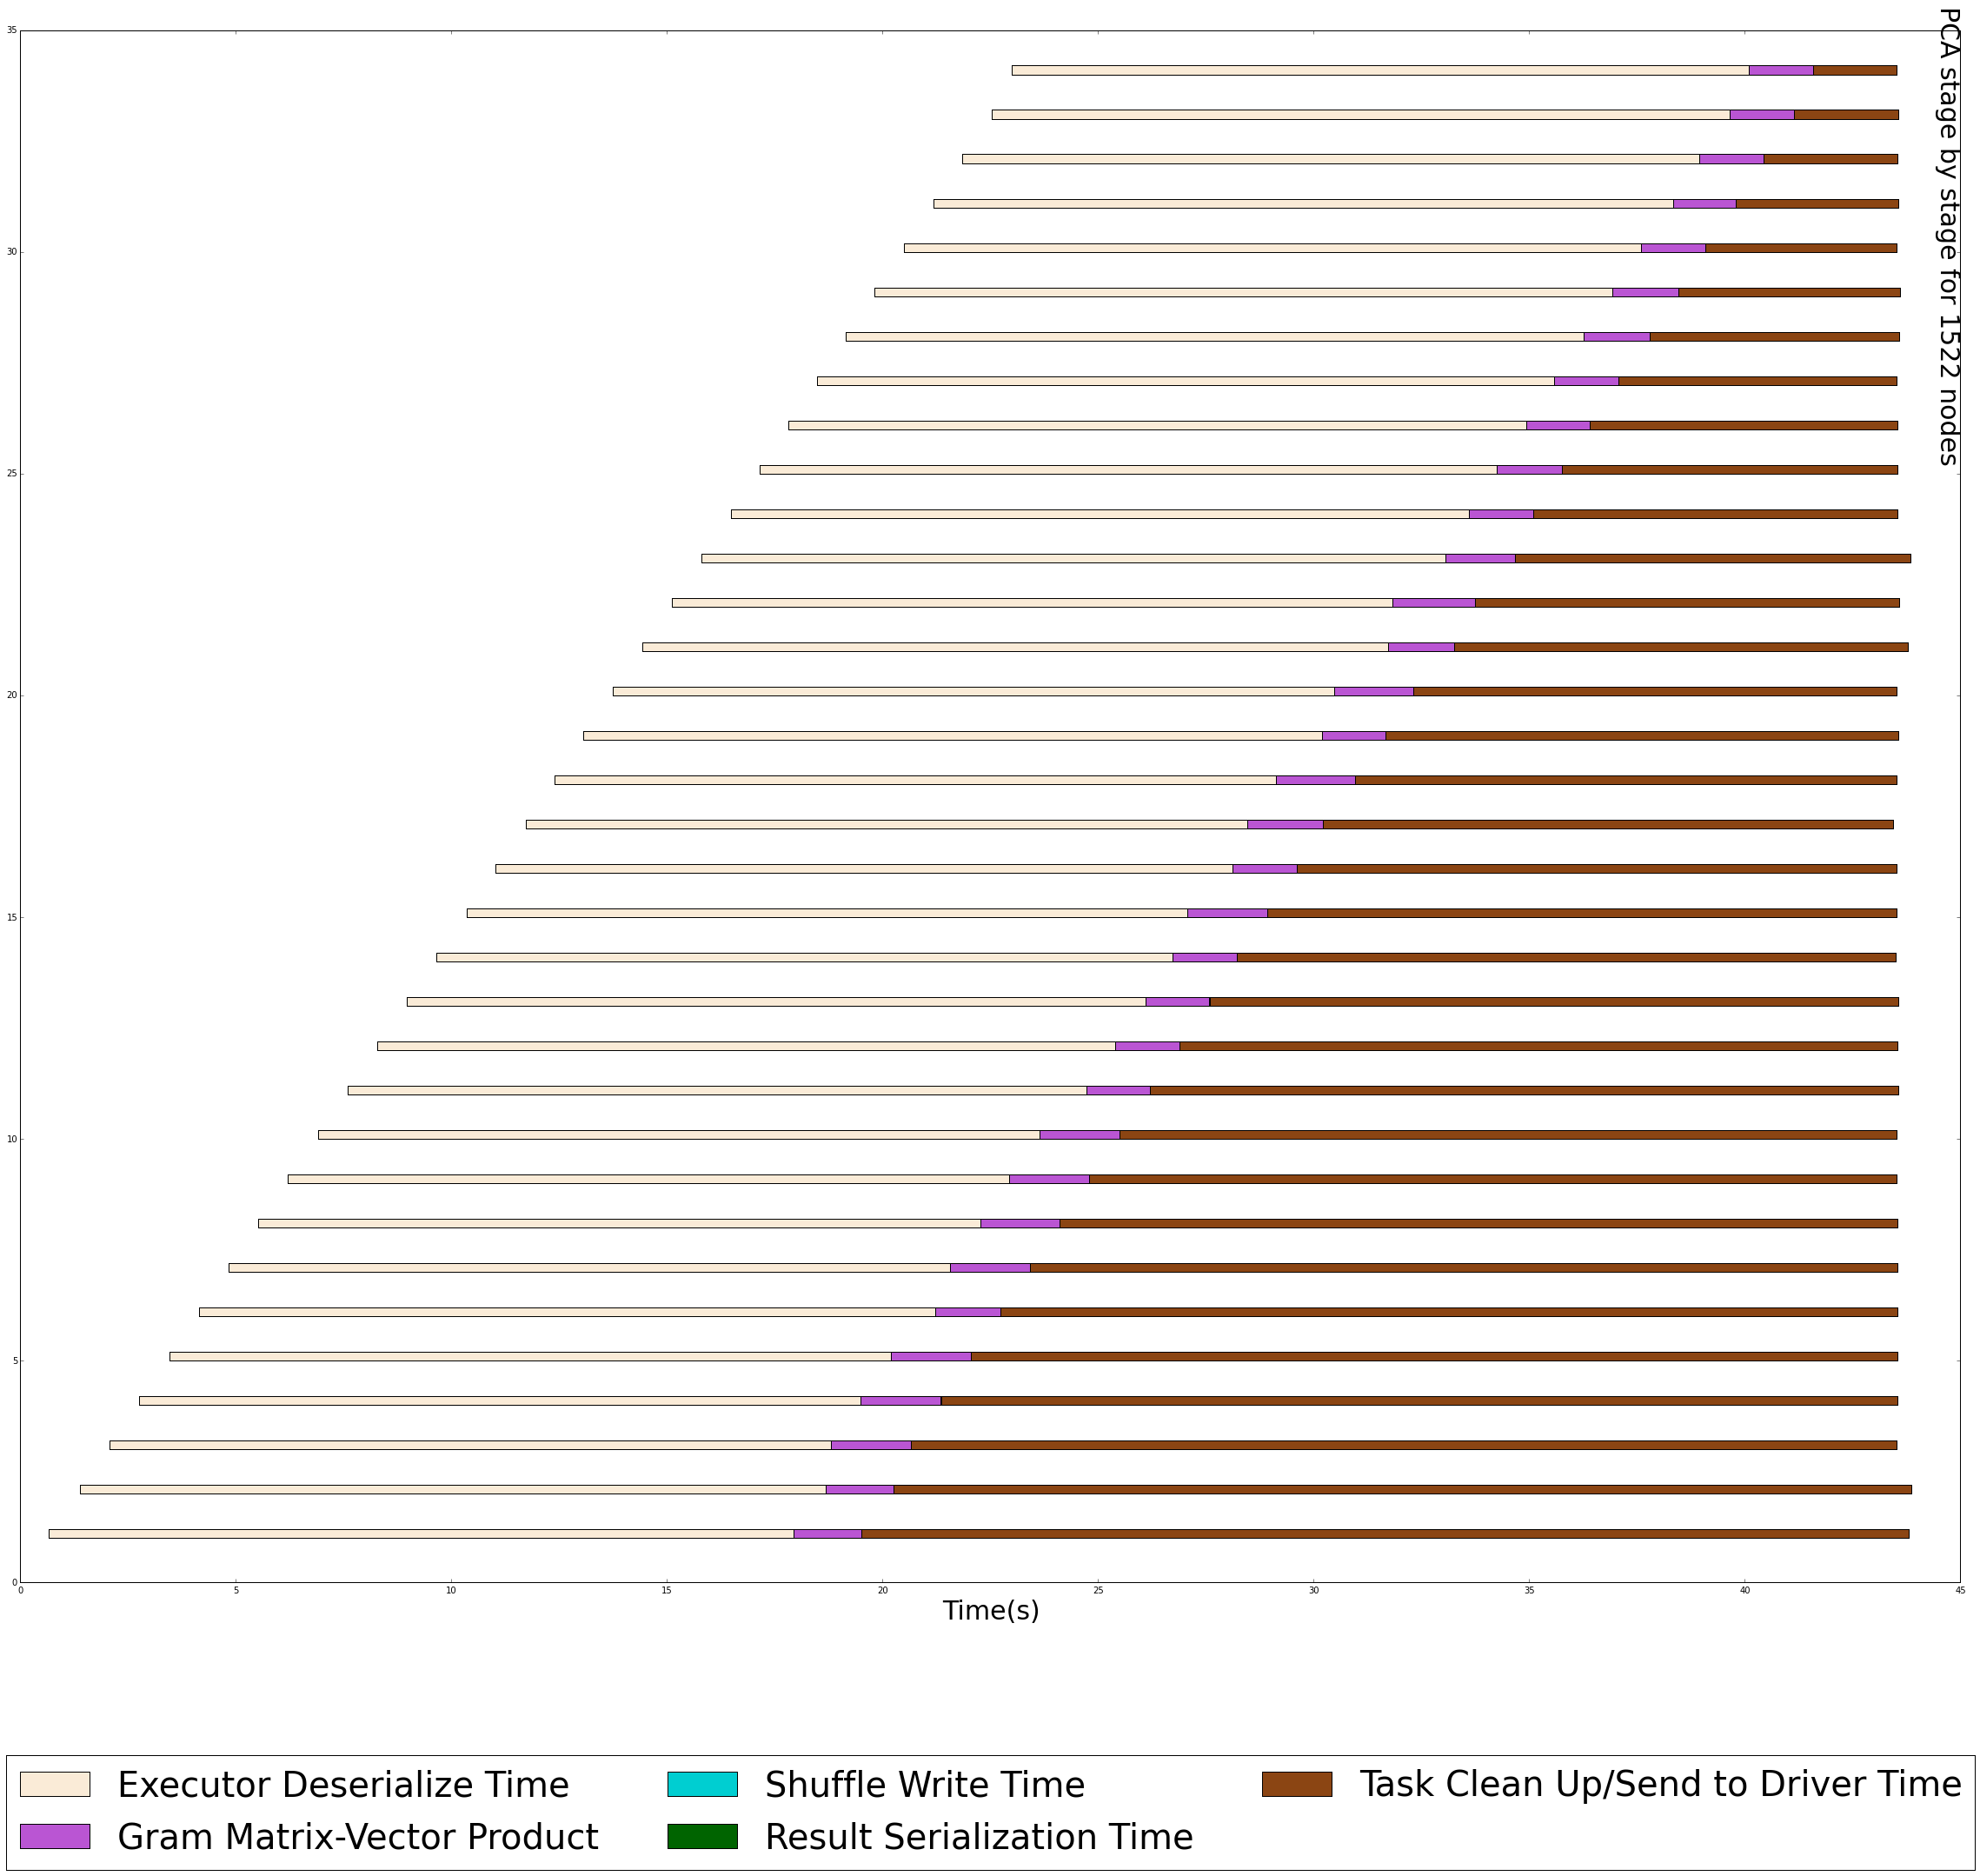
\includegraphics[width=.5\textwidth]{fig/pca_hero_timeline.png}
% \caption{???}
% \label{fig:tofix-3}
% \end{figure}

% \begin{figure}[t]
% 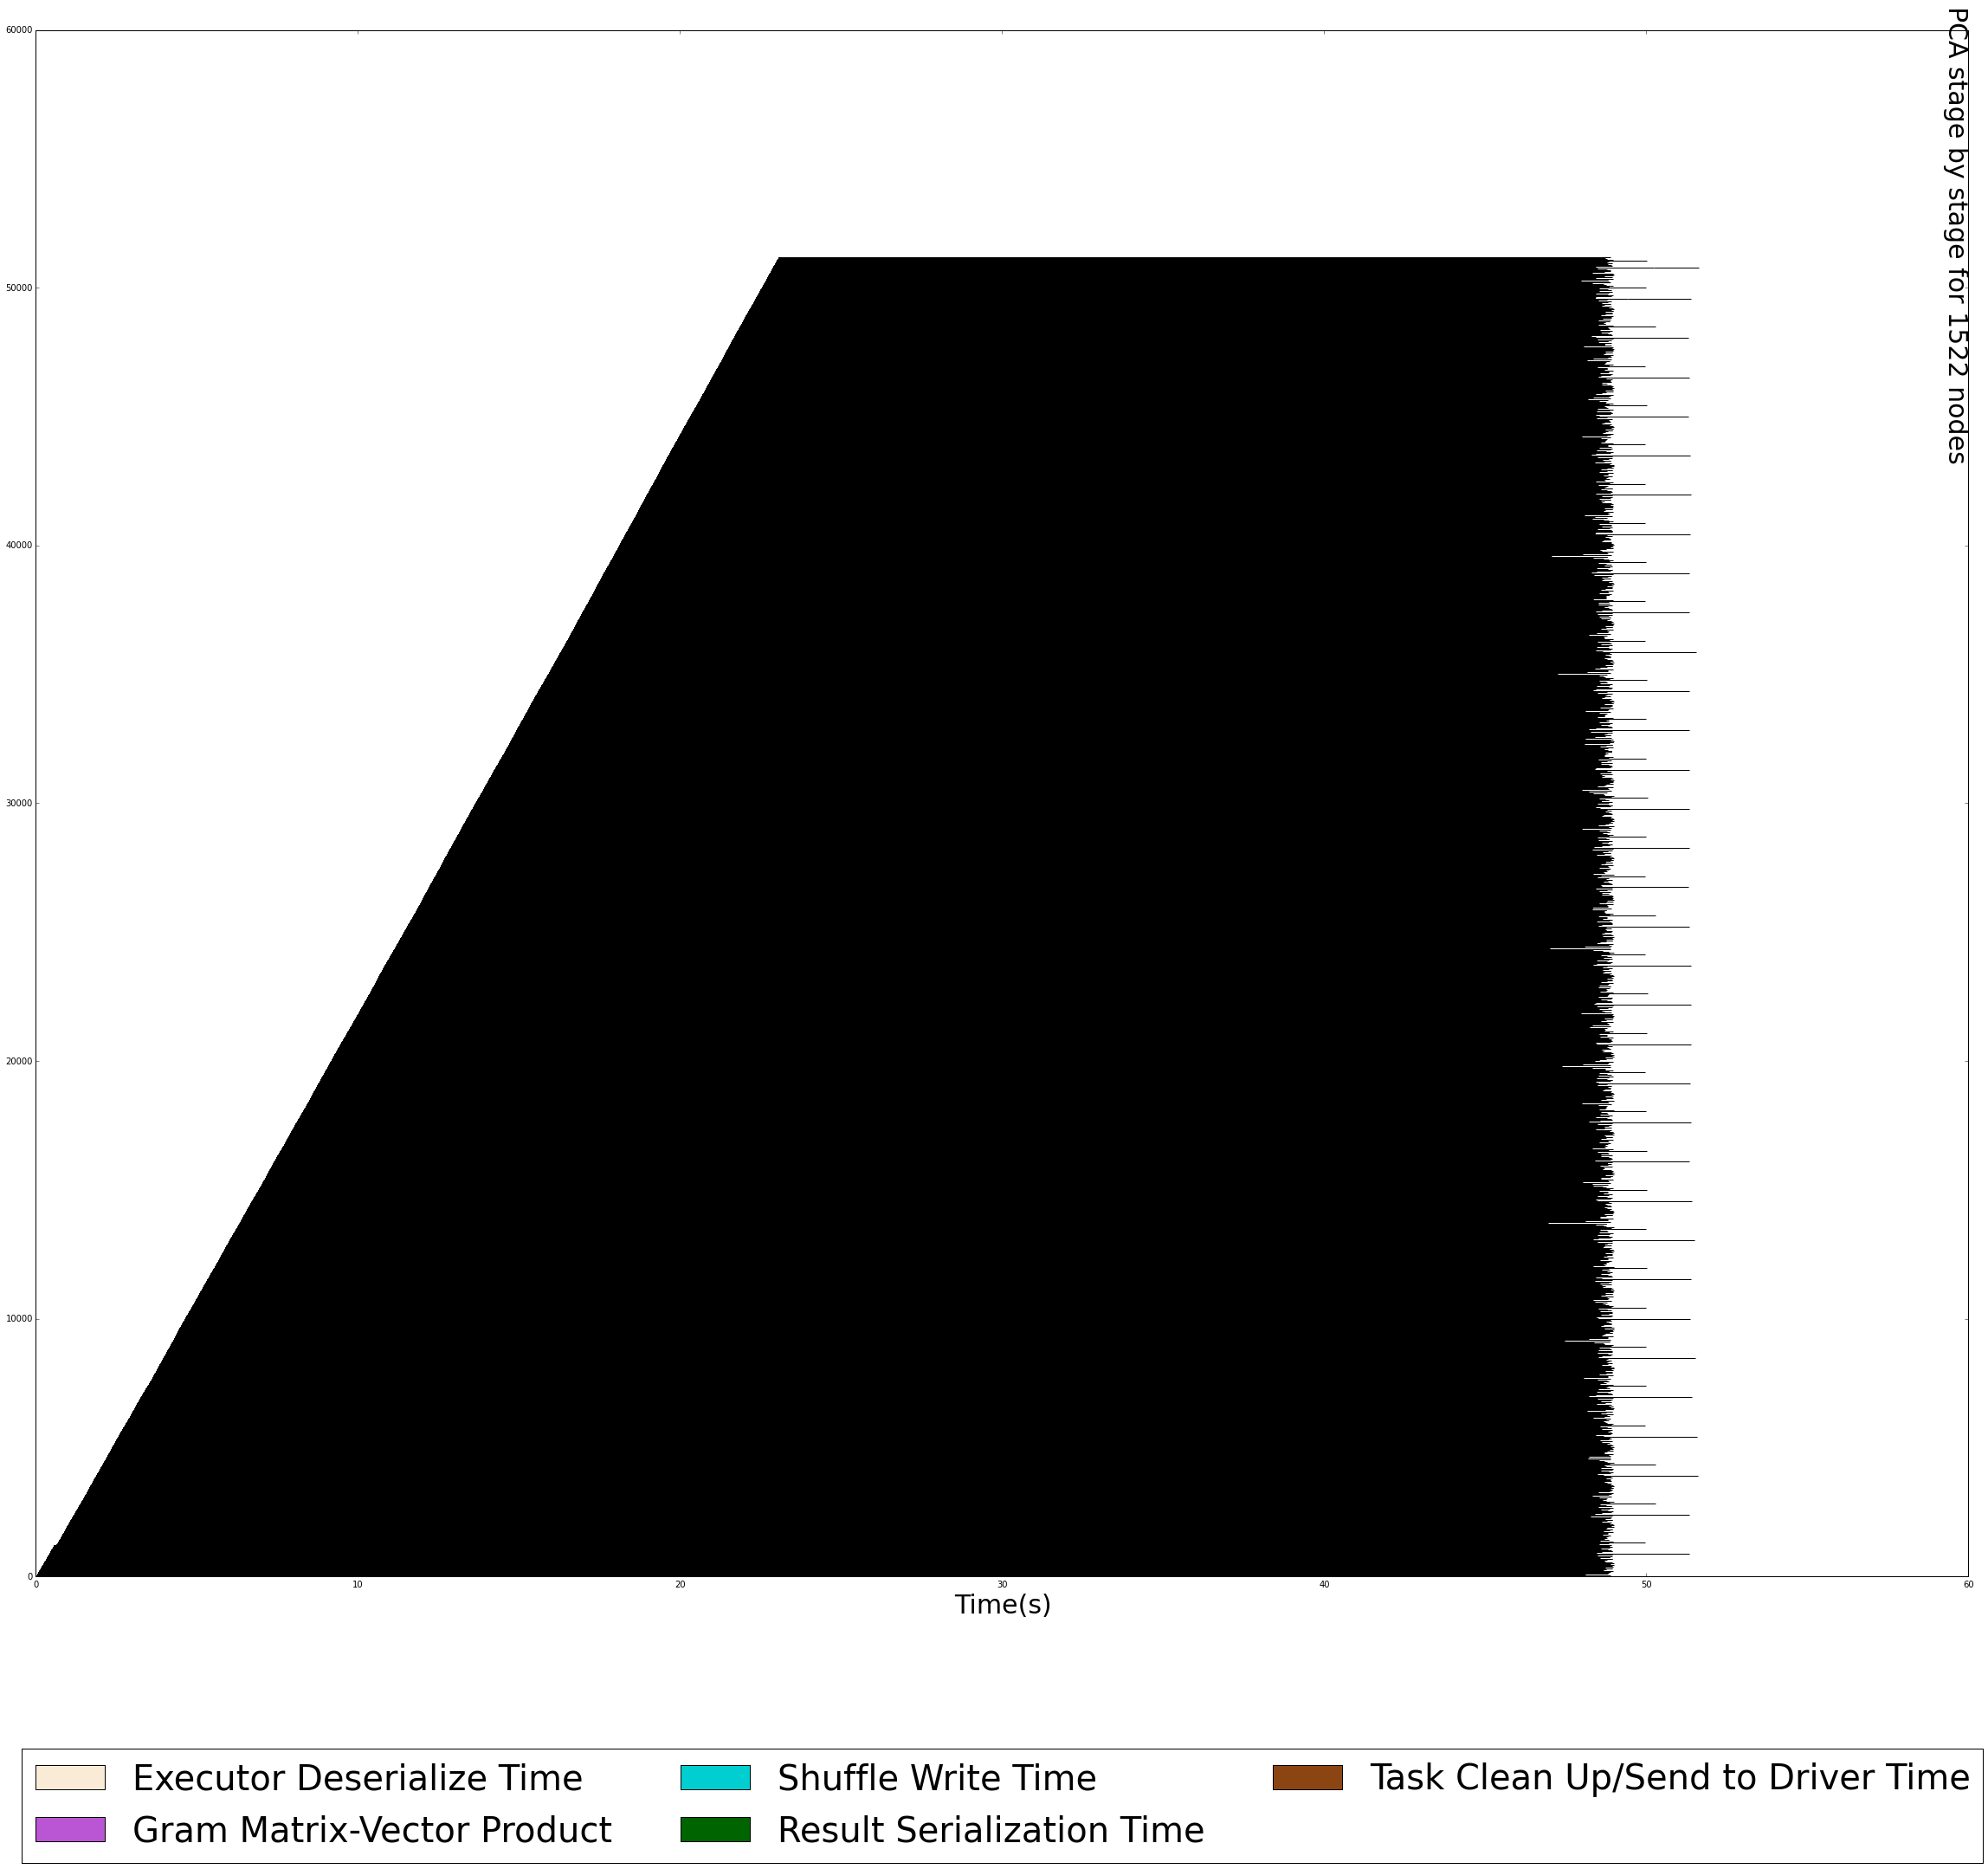
\includegraphics[width=.5\textwidth]{fig/stage7_hero_run.png}
% \caption{???}
% \label{fig:tofix-4}
% \end{figure}

\begin{figure}[t]
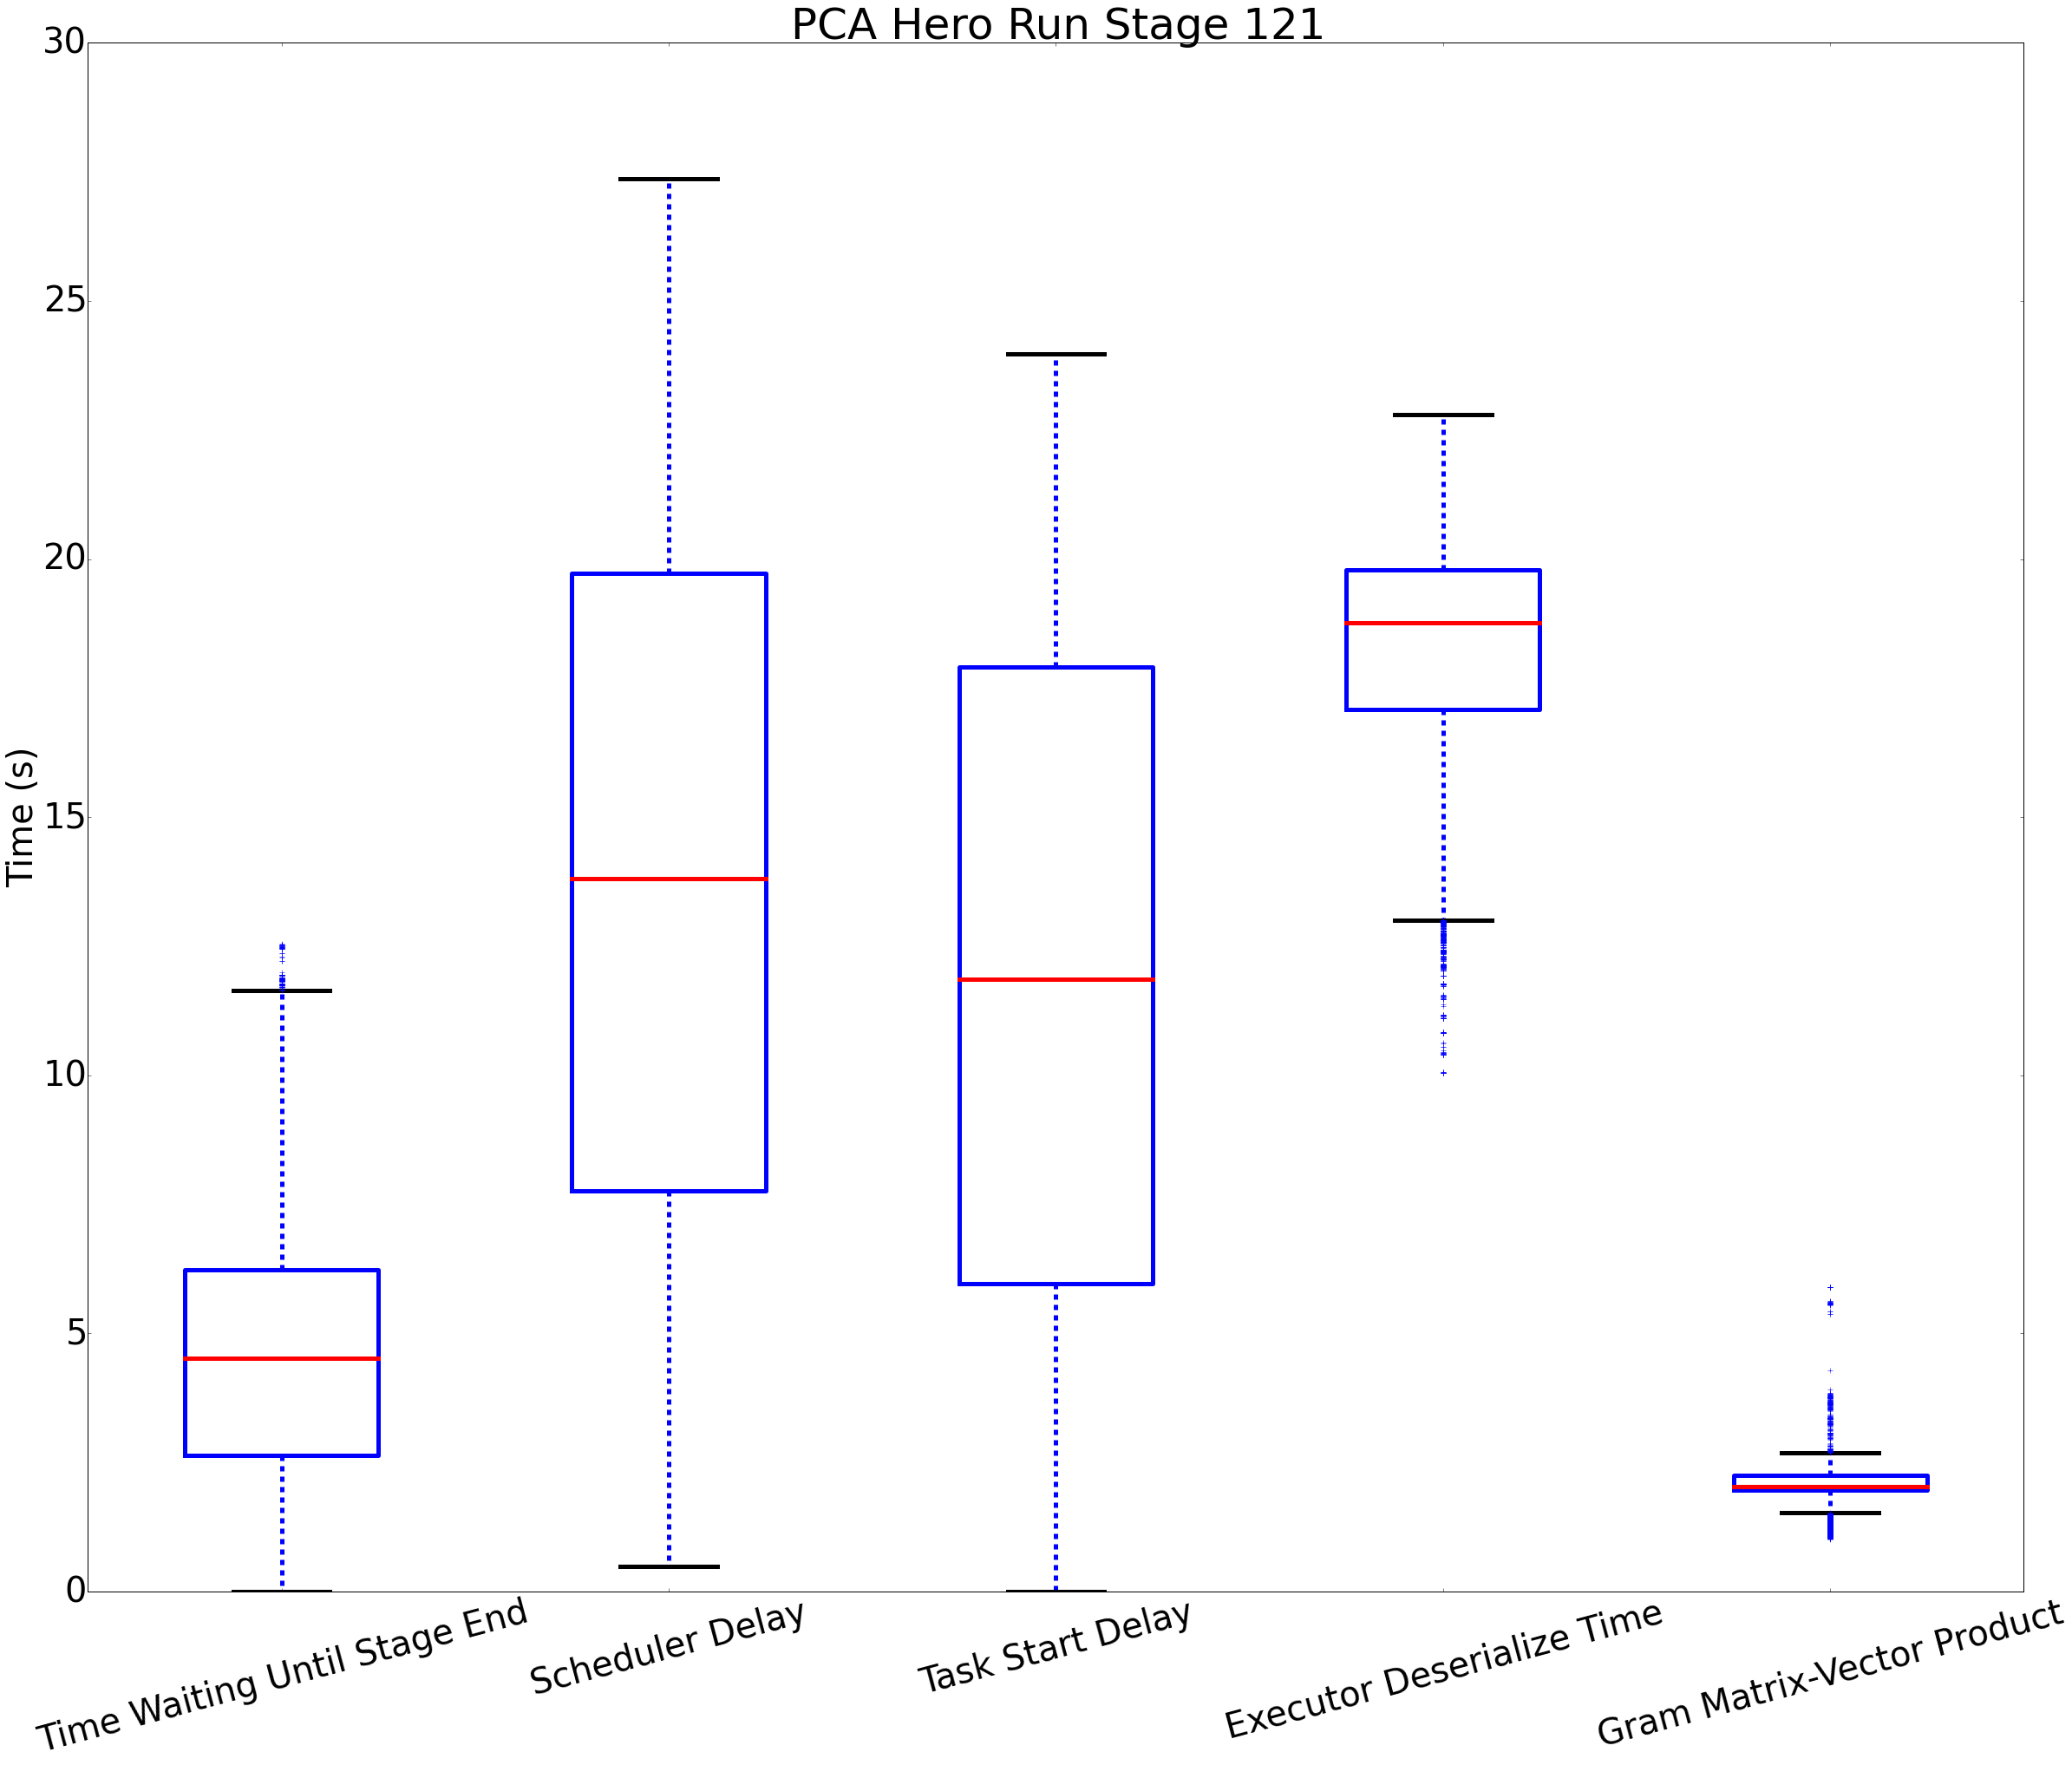
\includegraphics[width=.5\textwidth]{fig/box_and_whiskers.png}
\caption{Distribution of various components of all tasks in a multiply gramian stage in the Spark PCA hero run }
\label{fig:tofix-5}
\end{figure}


